%
% tsunami.tex -- XXX
%
% (c) 2011 Prof Dr Andreas Mueller, Hochschule Rapperswil
%

\section{Application: Wave propagation on a sphere or the tsunami of 2011}
\index{Tsunami}
On march 11 2011, an magnitude 9 earthquake in the japanese sea,
somtimes also referred to as the Sendai earthquake, triggered a 
tsunami that devastated large areas of the coast of the japanese
Fukushima province.
More than 15000 people were killed and multiple nuclear plants
were impacted, of which the the Fukushima-Daichi plant with a
a partial core meltdown was the most serious.
Tsunamis are waves triggered by earthquakes.
They are hardly noticeable in the open ocean and travel quite fast
but grow dramatically when the approach shallow waters near the coast.
The propagation of waves can modelled with a wave equation as has
been presented in chapter~\ref{chapter:examples}, but usually with
a propagation speed dependent on the depth of the ocean.
Figures \ref{tsunamiausbreitung} and \ref{tsunamienergie}
show the propagation of the wave caused by the Sendai earthquake
computed with the help of a computer.
It is obvious that the topography of the sea floor has a significant
influence on the propagation.

This makes a manual computation of the wave propagation almost
impossible, we would have to completely model the ocean floor and
the details of the coastline.
As a simplified model, we can try to understand the propagation of a
wave on an ocean covering a sphere with constant depth.

\begin{figure}
\begin{center}
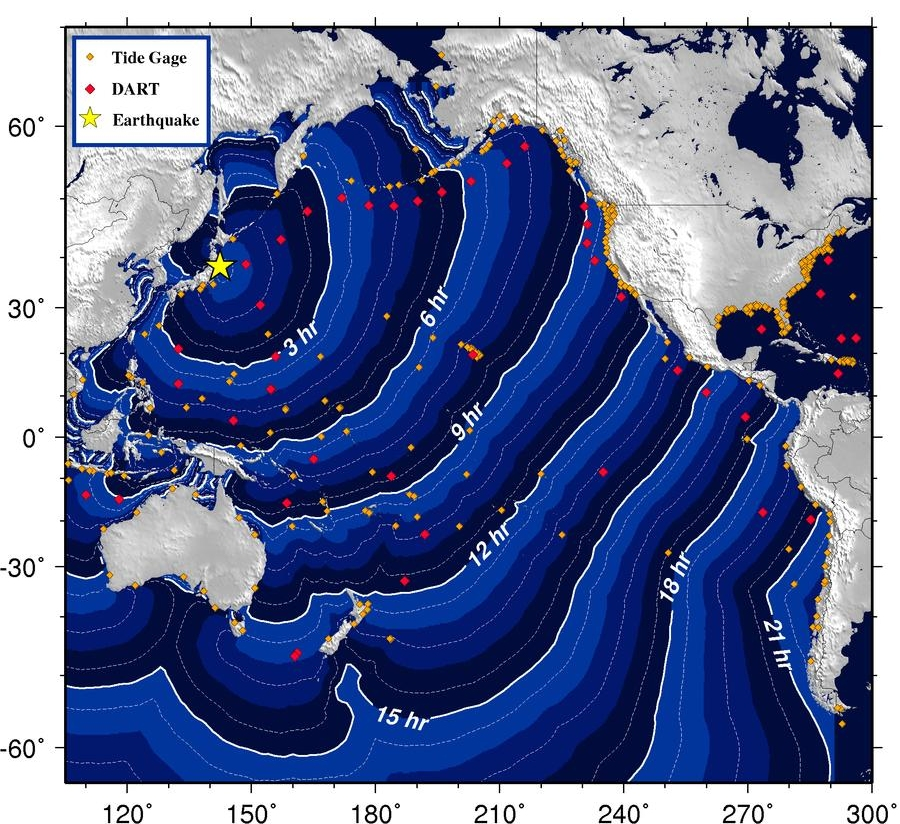
\includegraphics[width=\hsize]{../common/graphics/sendainoaa}
\end{center}
\caption{
Propagation of the tsunami caused by the Sendai earthquake on march 11 2011
based on a simulation by NOAA.
Hawai and other islands reduce the depth and thus the speed of propagation
of the wave.
Also apparent the shadowing of the wave due to obstacles like New Zealand.
\label{tsunamiausbreitung}}
\end{figure}

\begin{figure}
\begin{center}
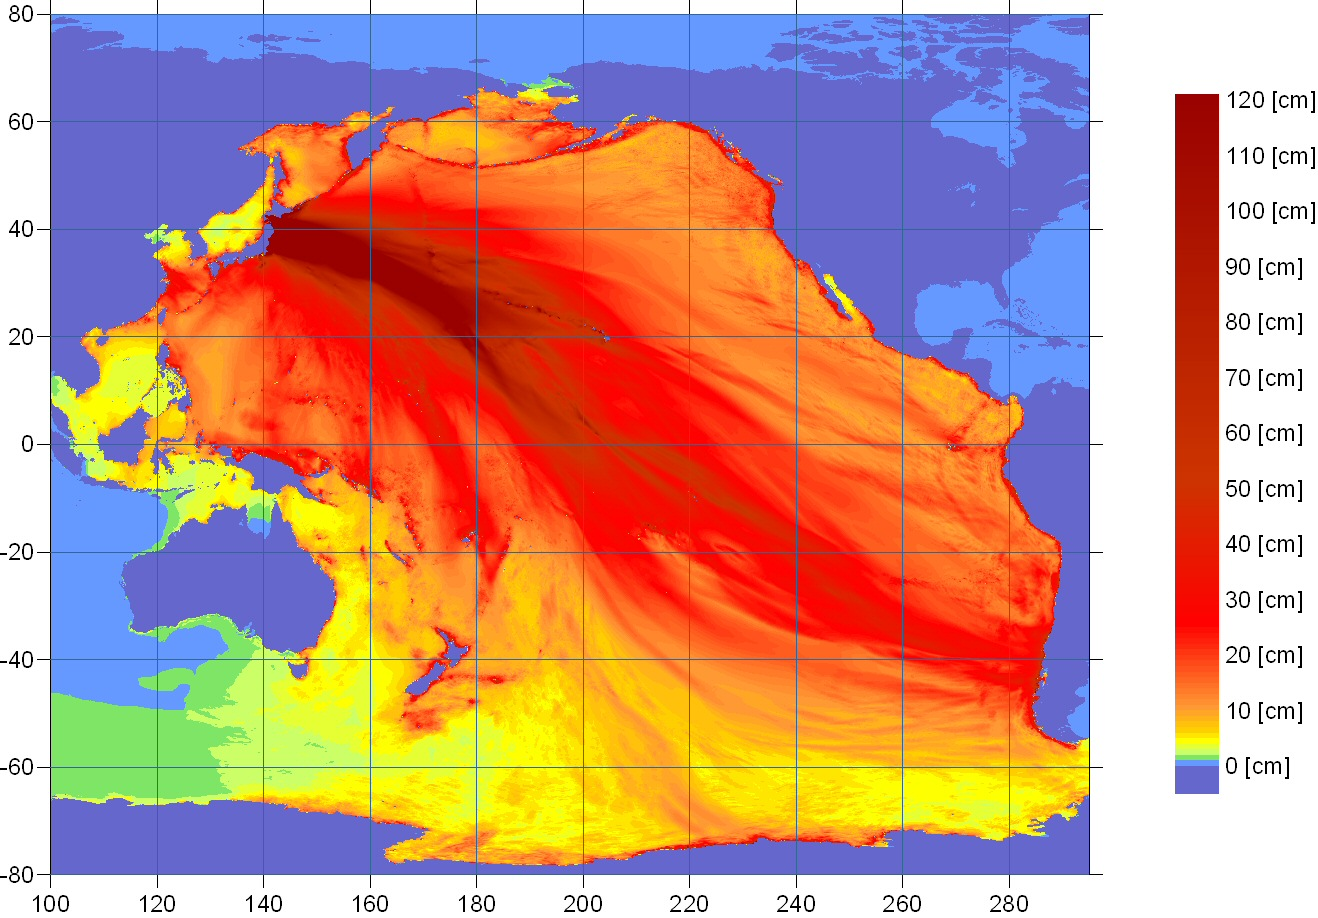
\includegraphics[width=\hsize]{../common/graphics/sendaienergy}
\end{center}
\caption{
Amplitude of the tsuname of march 11 2011.
Note that the great circles along which the waves propagate are mapped
to S-shaped durves.
Close to the coast the amplitude increases because of the reduced depth
and thus reduced velocity.
\label{tsunamienergie}}
\end{figure}

\subsection{Coordinates and boundary conditions}
We are interested in a wave originating in a single point, the
epicenter of the earthquake.
The solution in the idealized situation will necessarily be rotationally
symmetric around the axis through the epicenter.

We use spherical coordinates $(r,\vartheta,\varphi)$.
$\vartheta$ is the latitude measured from the north pole which will
also be the epicenter.
$\varphi$ is the longitude, a rotationally symmetric wave will not
depend on $\varphi$.
We can also neglect the $r$, as we consider only what happens at the
surface.
We therefore set $r=1$.

We are looking for a function
$u(t,\vartheta)$ satisfying initial conditions
\begin{align*}
u(0,\vartheta)&=F(\vartheta)\\
\frac{\partial}{\partial t}u(0,\vartheta)&=G(\vartheta).
\end{align*}

\subsection{Wave equation on the surface of a sphere}
The wave equation on the surface of a sphere can be obtained
by restricting the three dimensional wave equation
\[
\frac1{c^2} \frac{\partial^2}{\partial t^2}u =\Delta u.
\]
to the surface of the sphere.
We assume that units are chosen so that $c=1$, which amounts
to setting the time unit to time it takes for the wave to travel
one earth radius.


Wir nehmen an, dass die Einheiten so gewählt worden sind,
dass $c=1$ in diesen Einheiten gilt (dies erreicht man zum
Beispiel, wenn man als Längeneinheit die in einer Zeiteinheit
zurückgelegte Strecke verwendet).
Der Laplace-Operator muss in Kugelkoordinaten ausgedrückt werden,
\index{Laplace-Operator!in Kugelkoordinaten}
\[
\Delta u
=
\frac1{r^2} \frac{\partial}{\partial r}r^2\frac{\partial}{\partial r}u
+
\frac1{r^2\sin\vartheta}
\frac{\partial}{\partial\vartheta}
\sin\vartheta
\frac{\partial}{\partial\vartheta}
u
+
\frac1{r^2\sin^2\vartheta}\frac{\partial^2}{\partial\varphi^2}u
=
\frac1{\sin\vartheta}
\frac{\partial}{\partial\vartheta}
\sin\vartheta
\frac{\partial}{\partial\vartheta}
u
\]
Die Wellengleichung lautet jetzt also noch
\begin{equation}
\frac{\partial^2u}{\partial t^2}=
\frac1{\sin\vartheta}
\frac{\partial}{\partial\vartheta}
\sin\vartheta
\frac{\partial}{\partial\vartheta}
u=0.
\label{tsunami-gleichung}
\end{equation}

\subsection{Separation}
Für die Lösung der Wellengleichung (\ref{tsunami-gleichung}) machen
wir jetzt den üblichen Separationsansatz:
\[
u(t,\vartheta)=T(t)\Theta(\vartheta),
\]
und setzen ihn in die Differentialgleichung ein:
\[
T''(t)\Theta(\vartheta)=
T(t)
\frac1{\sin\vartheta}
\frac{d}{d\vartheta}
\sin\vartheta
\frac{d}{d\vartheta}\Theta(\vartheta)
\]
Da wir eine Lösung suchen, die nicht überall verschwindet,
dürfen wir annehmen, dass $T$ und $\Theta$ ausser an einzelnen
Punkten nicht verschwinden, dass wir also ``meistens'' durch
$T(t)\Theta(\vartheta)$ teilen dürfen. Damit erreichen wir
die gewünschte Trennung der Variablen:
\begin{equation}
\frac{T''(t)}{T(t)}
=
\frac1{\Theta(\vartheta)}
\frac1{\sin\vartheta}
\frac{d}{d\vartheta}
\sin\vartheta
\frac{d}{d\vartheta}\Theta(\vartheta)
\label{tsunami-separiert}
\end{equation}
Die linke Seite ist nur von $t$ abhängig, die rechte nur von $\vartheta$,
diese Gleichung kann also nur erfüllt sein, wenn beide seiten konstant
sind.  Wir erhalten also zwei Gleichungen
\begin{align}
T''(t)&=mT(t)
\label{tsunami:zeitabh}
\\
\frac1{\sin\vartheta}
\frac{d}{d\vartheta}
\sin\vartheta
\frac{d}{d\vartheta}\Theta(\vartheta)
&=m\Theta(\vartheta).
\label{tsunami:winkelabh}
\end{align}
Es ist jetzt also zu ermitteln, für welche Werte von $m$ die beiden
Gleichungen Lösungen haben. Dann können für diese Werte von $m$ 
Lösungen der partiellen Differentialgleichung zusammengebaut werden,
mit denen sich dann beliebige Lösungen durch Überlangerungen
erfüllen lassen müssen.

\subsection{Zeitabhängigkeit}
Die Zeitabhängigkeit (\ref{tsunami:zeitabh}) ist eine gewöhnliche
Schwingungsdifferentialgleichung.
Die Lösungen sollten Schwingungscharakter haben, was nur zutrifft, wenn
$m<0$ ist. Die allgemeine Lösung ist dann
\[
T_m(t)=a_m\cos\sqrt{-m}t+b_m\sin\sqrt{-m}t
\]

\subsection{Winkelabhängigkeit}
Die Differentialgleichung (\ref{tsunami:winkelabh}) für $\Theta$
ist in dieser Form etwas unhandlich.
Daher ersetzen wir $\Theta(\vartheta)$ durch eine
Funktion $y(x)$ mit Hilfe der Substitution $x=\cos\vartheta$.
Die Ableitung nach $\vartheta$ kann mit Hilfe der Kettenregel
in eine Ableitung nach $x$ umgewandelt werden:
\[
\frac{d}{d\vartheta}\Theta(\vartheta)
=\frac{dy(x)}{dx}\frac{dx}{d\vartheta}
=-\sin\vartheta \frac{d}{dx} y(x)
\]
Setzt man dies in die Differentialgleichung ein, wird sie zu
\begin{align*}
\frac1{\sin\vartheta}
(-\sin{\vartheta})\frac{d}{dx}\sin\vartheta (-\sin\vartheta)
\frac{d}{dx}y(x)
&=
\frac{d}{dx}\sin^2\vartheta\frac{d}{dx}y(x)\\
&=
\frac{d}{dx}(1-\cos^2\vartheta)\frac{d}{dx}y(x)\\
&=
\frac{d}{dx}(1-x^2)\frac{d}{dx}y(x).
\end{align*}
Die gesuchten Funktionen sind also Lösungen der Differentialgleichung
\begin{equation}
\frac{d}{dx}(1-x^2)\frac{d}{dx}y(x)
=
my(x)
\label{tsunamieigenwertproblem}
\end{equation}
Die Funktionen $y(x)$ müssen im ganzen Interval $[-1,1]$ definiert
sein. Dies ist nicht unbedingt selbstverständlich, wie schon der Fall
$m=0$ zeigt. In diesem Fall kann man die Differntialgleichung
durch zweimaliges Integrieren lösen:
\begin{align*}
\frac{d}{dx}(1-x^2)\frac{d}{dx}y(x)&=0\\
(1-x^2)\frac{d}{dx}y(x)&=C\\
\frac{d}{dx}y(x)&=\frac{C}{1-x^2}\\
y(x)&=C\int\frac{dx}{1-x^2}\\
&=\frac{C}2\int\frac{dx}{1-x}+\frac{C}2\int\frac{dx}{1+x}\\
&=-\frac{C}2\log(1-x)+\frac{C}2\log(1+x) +D\\
&=\frac{C}2\log\frac{1+x}{1-x} + D
\end{align*}
An beiden Intervallenden wächst die Funktion über alle Grenzen,
es sei denn es sei $C=0$.

Mit Sicherheit auf dem ganzen Interval definiert wären Polynome,
wir könnten also einen Ansatz
\[
y(x)=a_0+a_1+a_2x^2+\dots a_nx^n
\]
probieren. Setzt man dies in die Differentialgleichung ein und
behält nur die Terme vom Grad $x^n$, bekommt man auf der rechten
Seite von (\ref{tsunamieigenwertproblem}) $ma_nx^n$, auf
der linken Seite
\[
-\frac{d}{dx}x^2\frac{d}{dx}a_nx^n
=
-\frac{d}{dx}x^2na_nx^{n-1}
=
-\frac{d}{dx}na_nx^{n+1}
=
-n(n+1)a_nx^n
\]
Damit folgt: $m=-n(n+1)$, nur für solche Werte kann
(\ref{tsunamieigenwertproblem}) ein Polynom vom Grad $n$ als Lösung
haben. Die Differentialgleichung wird jetzt zu
\begin{equation}
\frac{d}{dx}(1-x^2)\frac{d}{dx}y(x)+n(n+1)y(x)=0
\label{legendredgl}
\end{equation}

\subsection{Legendre-Polynome}
\index{Legendre-Polynom}
Die Differentialgleichung (\ref{legendredgl}) ist die Differentialgleichung
der Legendre-Polynome.
Das Legendre-Polynom $P_n(x)$ ist eine polynomiale Lösung von
(\ref{legendredgl}) mit $P_n(1)=1$.
Dies legt aber die Funktion nicht fest, es sind weitere Bedingungen
nötig. Daher wird verlangt, dass die Polynome auch orthogonal
sein sollen, also die Bedingung
\[
\int_{-1}^1 P_k(x)P_l(x)\,dx=0\quad\text{für $k\ne l$}
\]
erfüllen. Damit werden die Polynome eindeutig.
Die ersten sechs Legendre-Polynome sind
\begin{align*}
P_0(x)&=1\\
P_1(x)&=x\\
P_2(x)&=\frac12(3x^2-1)\\
P_3(x)&=\frac12(5x^3-3x)\\
P_4(x)&=\frac18(35x^4-30x^2+3)\\
P_5(x)&=\frac18(63x^5-70x^3+15x)
\end{align*}
Ausserdem gilt
\[
\int_{-1}^1 P_k(x)^2\,dx = \frac{2}{2k+1}.
\]
Da man 
jede Funktion auf dem Interval $[-1,1]$ mit Polynomen approximieren kann,
kann man auch jede Funktion durch Linearkombinationen von Legendre-Polynomen
$P_n(x)$ schreiben. 

Die Koeffizienten kann man mit Hilfe eines Integrals finden. Setzt man
\[
f(x)=\sum_{k\ge 0} c_k P_k(x)
\]
und berechnet man das Integral
\[
\int_{-1}^1 f(x)P_l(x)\,dx
=
\sum_{k\ge 0} c_k \int_{-1}^1 P_k(x)P_l(x)\,dx
=
\frac{2c_k}{2k+1}
\]
folgt
\[
c_k=\frac{2k+1}{2}\int_{-1}^1P_k(x)f(x)\,dx.
\]
Die Koeffizienten $c_k$ sind sozusagen die ``Legendre-Koeffizienten''
der Entwicklung der Funktion $f(x)$ nach Legendre-Polynomen,
analog zu den Fourier-Koeffizienten auf einem Interval.

\subsection{Anfangsbedingungen}
\index{Anfangsbedingungen}
Unter Verwendung der Legendre-Polynome kann man jetzt die Wellengleichung
zu beliebigen Anfangsbedingungen lösen.
Die Lösung der Differentialgleichung muss von der Form sein
\[
u(t, x)=\sum_{k=0}^{\infty}(a_k\cos \lambda_k t+b_k\sin\lambda_k t)P_k(x),
\]
wobei $\lambda_k=\sqrt{k(k+1)}$.
Die Koeffizienten müssen aus der Anfangsbedingung, also aus den 
Funktionen $F(\vartheta)=f(x)$ und $G(\vartheta)=g(x)$ bestimmt werden.
Die Anfangsbedingung für $u(t,x)$ ergibt
\begin{align*}
u(0,x)
&=\sum_{k=0}^{\infty} a_kP_k(x)=f(x)
\end{align*}
Für $\partial_tu(t,x)$ ergibt sich entsprechend
\begin{align*}
\frac{\partial}{\partial t}u(0,x)
&=\sum_{k=0}^{\infty} \lambda_k b_kP_k(x)=g(x)
\end{align*}
Die Koeffizienten $a_k$ und $b_k$ kann man mit
\begin{align*}
a_k&=
\frac{2k+1}{2}\int_{-1}^1 P_k(x)f(x)\,dx
\\
b_k&=
\frac{2k+1}{2\lambda_k}\int_{-1}^1P_k(x)f(x)\,dx
\end{align*}
berechnen.

\subsection{Punktquelle}
\begin{figure}
\begin{center}
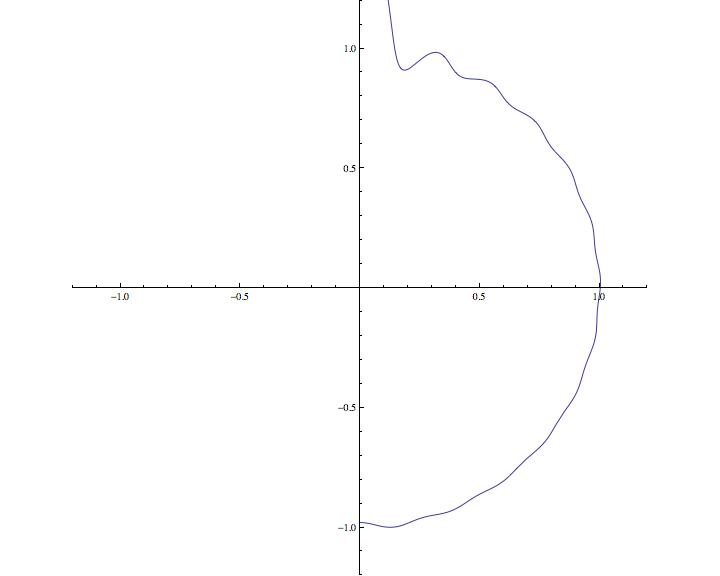
\includegraphics[width=\hsize]{../common/graphics/tsunami0}
\end{center}
\caption{Näherungslösung für $N=25$ und $t=0$\label{tsunami0}}
\end{figure}
\begin{figure}
\begin{center}
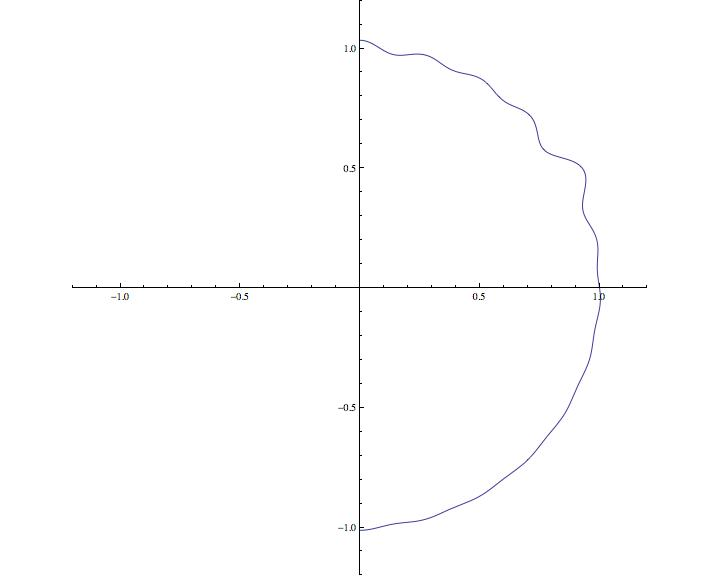
\includegraphics[width=\hsize]{../common/graphics/tsunami50}
\end{center}
\caption{Näherungslösung für $N=25$ und $t=1$\label{tsunami50}}
\end{figure}

Wir wählen jetzt eine spezielle Anfangsbedingung:
\begin{align*}
f_\varepsilon(x)&=\begin{cases}
\frac1{\varepsilon}&\qquad 1-\varepsilon<x\le 1\\
0&\qquad\text{sonst}
\end{cases}
\\
g(x)&=0
\end{align*}
In einer kleinen Umgebung des Nordpoles ist der Wert 
$\frac1{\varepsilon}$, also sehr gross, in allen anderen Punkten $0$.
Offenbar sind die $b_k=0$, und es bleiben nur die 
$a_k$ zu berechnen. Dazu gilt:
\begin{align*}
a_k(\varepsilon)&=\frac{2k+1}{2}\int_{-1}^1P_k(x)f_\varepsilon(x)\,dx
\\
&=\frac{2k+1}{2}\int_{1-\varepsilon}^1P_k(x)\frac1{\varepsilon}\,dx
\end{align*}
Da uns nur der Grenzwert $\varepsilon\to 0$ interessiert, gehen wir
zur Grenze über
\begin{align*}
\lim_{\varepsilon\to 0} a_k(\varepsilon)
&=
\frac{2k+1}{2}\lim_{\varepsilon\to 0}\frac1{\varepsilon}\int_{1-\varepsilon}^1P_k(x)\,dx
\end{align*}
Mit einer Stammfunktion $I_k(x)$ von $P_k(x)$ wird dies zu
\begin{align*}
\lim_{\varepsilon\to 0} a_k(\varepsilon)
&=
\frac{2k+1}{2}\lim_{\varepsilon\to 0}\frac{I_k(1)-I_k(1-\varepsilon)}{\varepsilon}
\\
&=\frac{2k+1}{2}I_k'(1)=\frac{2k+1}{2}P_k(1)=\frac{2k+1}{2}
\end{align*}
Als Lösung bekommt man damit formal
\begin{equation}
u(t,x)
=
\sum_{k=0}^\infty \frac{2k+1}{2}P_k(x) \cos \sqrt{k(k+1)}t.
\end{equation}
Leider ist diese Reihe nicht konvergent, was angesichts der sehr
speziellen Anfangsbedingungen auch nicht zu erwarten war.
Wenn man sie aber nach $N$ Termen abbricht, und mit $\frac1{N^2}$ 
normiert, erhält man eine Lösungsfunktion die ein ungefähres
Bild für die Wellenausbreitung ergibt.
In den Abbildungen \ref{tsunami0} und \ref{tsunami50} wurde die Reihe nach 25 Termen
abgebrochen.
